\documentclass[aspectratio=169]{beamer}
\usepackage{color,amsmath}
\usepackage{subfigure}
\usepackage{booktabs}
\usepackage{framed}
\usepackage{comment}

\def\vf{\vfill}

%%%%%%%%%%%%%%%%%%%%%%%%%%
\title[]{Computer-administered interviews\\(03-04)}
\author[]{Matthew J. Salganik\\Department of Sociology\\Princeton University}
\date[]{Soc 596: Computational Social Science\\Fall 2016
\vfill
\begin{flushright}
\vspace{0.6in}

\includegraphics[width=0.1\textwidth]{figures/cc.png}
\end{flushright}
}
\begin{document}
%%%%%%%%%%%%%%%%%%%%%%%%%%
\frame{\titlepage}
%%%%%%%%%%%%%%%%%%%%%%%%%%
\begin{frame}

\begin{center}
\small{
\begin{tabular}{ l c c c}
           & Sampling & Interviews & Data environment\\
\hline
1st era & Area probability & Face-to-face & Stand-alone \\
2nd era & \parbox[t]{3cm}{\centering Random digital dial\\probability} & Telephone & Stand-alone \\
3rd era & Non-probability & \textcolor{blue}{Computer-administered} & Linked \\
\end{tabular}
}
\end{center}

\end{frame}
%%%%%%%%%%%%%%%%%%%%%%%%%%%
\begin{frame}

\begin{center}
Human-administered $\rightarrow$ Computer-administered
\end{center}

\begin{itemize}
\item enables change
\item requires change
\end{itemize}

\end{frame}
%%%%%%%%%%%%%%%%%%%%%%%%%%
\begin{frame}
\frametitle{}
\begin{center}
\includegraphics<1>[width=3.5in]{figures/kittenwar_front_1_cut}
\includegraphics<2>[width=3.5in]{figures/kittenwar_front_2_cut}
\includegraphics<3>[width=3.5in]{figures/kittenwar_front_3_cut}
\end{center}
\end{frame}
%%%%%%%%%%%%%%%%%%%%%%%%%%%
\begin{frame}
\begin{center}
\begin{tabular}{ccc}
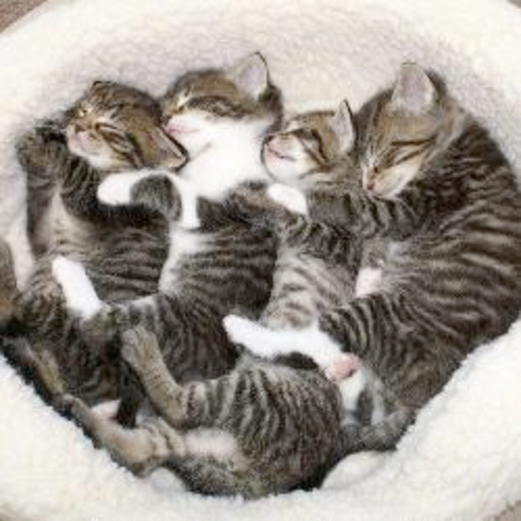
\includegraphics[width=1.2in]{figures/kittenwar_cute_1} & 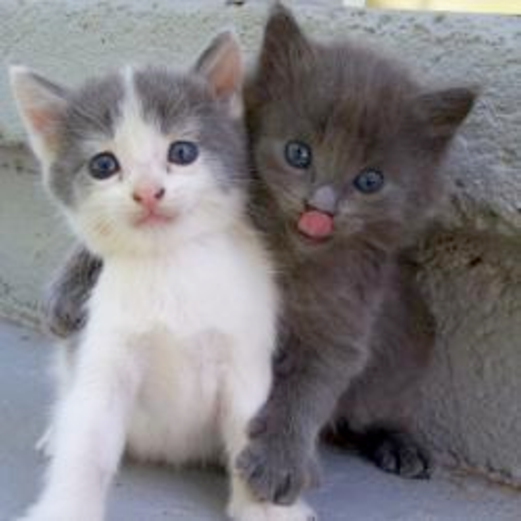
\includegraphics[width=1.2in]{figures/kittenwar_cute_2} & 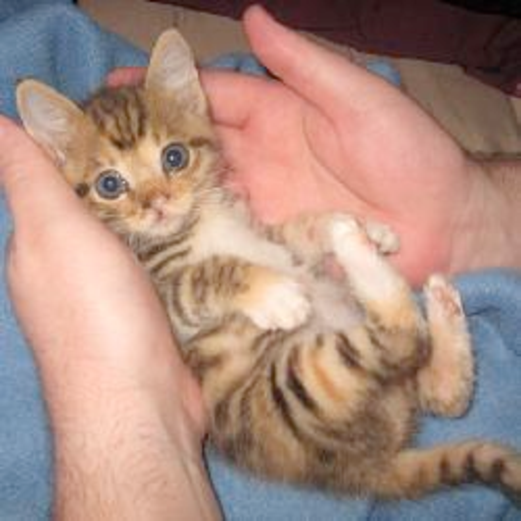
\includegraphics[width=1.2in]{figures/kittenwar_cute_3}\\
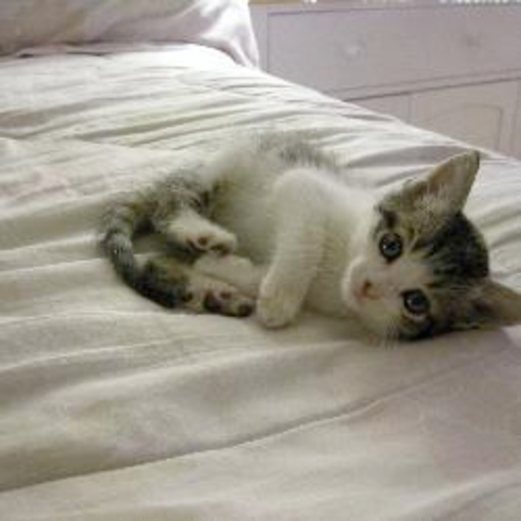
\includegraphics[width=1.2in]{figures/kittenwar_cute_4} & 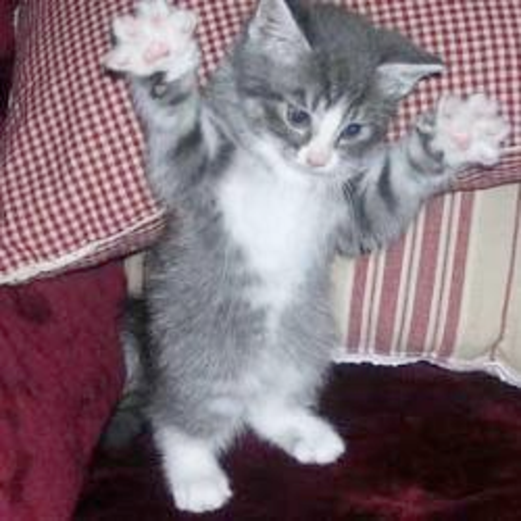
\includegraphics[width=1.2in]{figures/kittenwar_cute_5} & 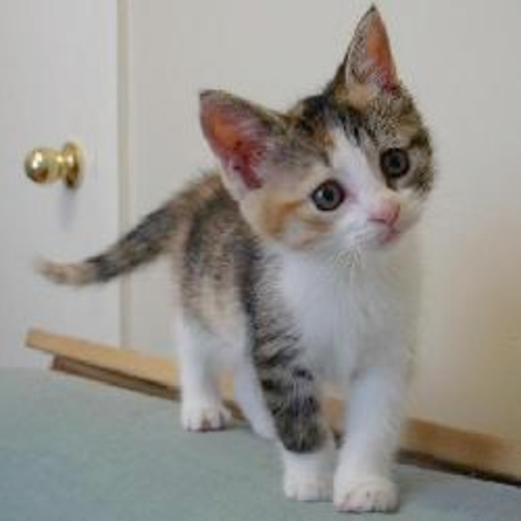
\includegraphics[width=1.2in]{figures/kittenwar_cute_6}
\end{tabular}
\end{center}
\end{frame}
%%%%%%%%%%%%%%%%%%%%%%%%%%%
\begin{frame}
\frametitle{}
\begin{center}
\begin{tabular}{ccc}
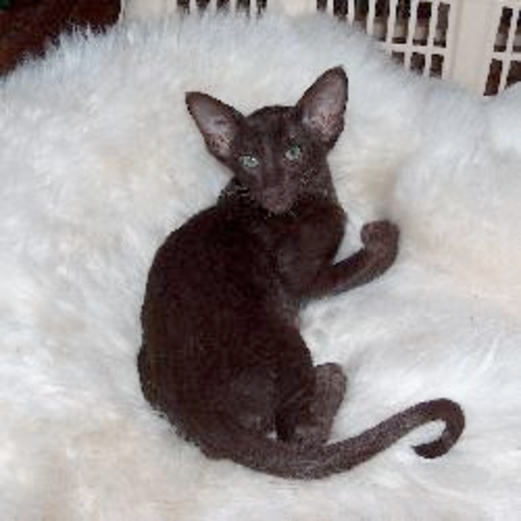
\includegraphics[width=1.2in]{figures/kittenwar_ugly_1} & 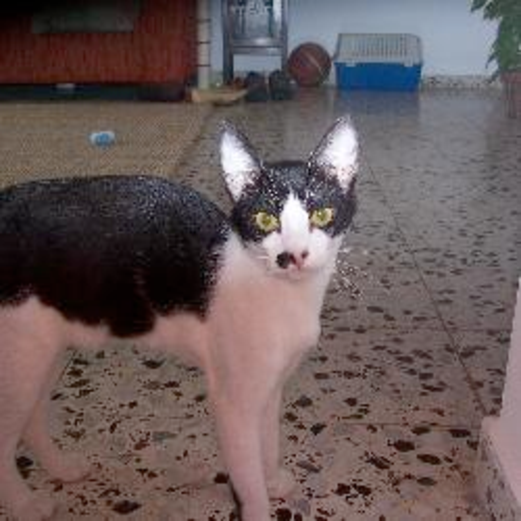
\includegraphics[width=1.2in]{figures/kittenwar_ugly_2} & 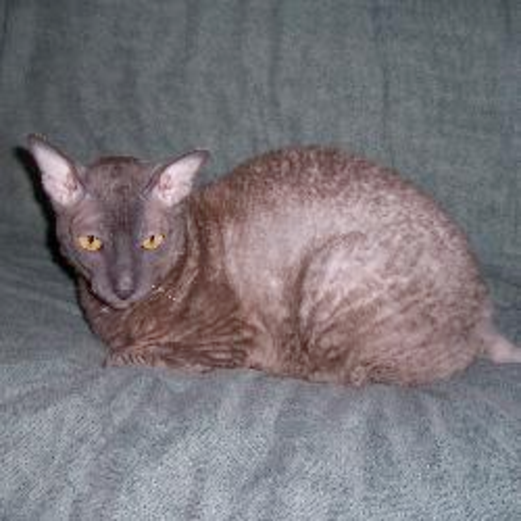
\includegraphics[width=1.2in]{figures/kittenwar_ugly_3}\\
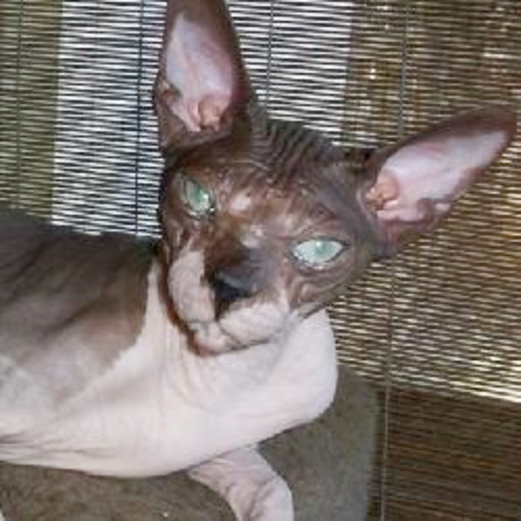
\includegraphics[width=1.2in]{figures/kittenwar_ugly_4} & 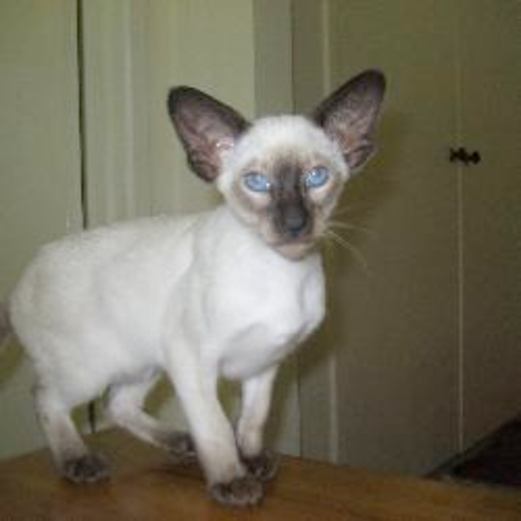
\includegraphics[width=1.2in]{figures/kittenwar_ugly_5} & 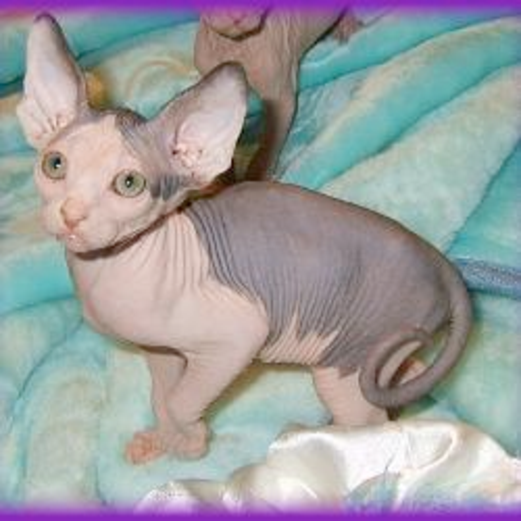
\includegraphics[width=1.2in]{figures/kittenwar_ugly_6}
\end{tabular}
\end{center}
\end{frame}
%%%%%%%%%%%%%%%%%
\begin{frame}

\begin{center}
{\LARGE quantification} or {\LARGE openness} 
\end{center}

\end{frame}
%%%%%%%%%%%%%%%%%
\begin{frame}

\begin{center}
{\LARGE quantification} + {\LARGE openness} =\\ \textcolor{blue}{\LARGE wiki surveys}
\end{center}

\end{frame}
%%%%%%%%%%%%%%%%%%%%%%%%%%
\begin{frame}

General principles of wiki surveys:
\begin{itemize}
\item greedy
\end{itemize}

\end{frame}
%%%%%%%%%%%%%%%%
\begin{frame}

\begin{columns}[c] 
\column{2.5in} 
\hspace{0.6in}Good web-based systems use\\ \hspace{0.6in}the \textcolor{blue}{fat-head} and the \textcolor{blue}{long-tail} 
\column{1in} 
\hspace{-0.3in}
\includegraphics[width=0.6in]{figures/200px-Wikipedia-logo}
\end{columns} 

\begin{center}
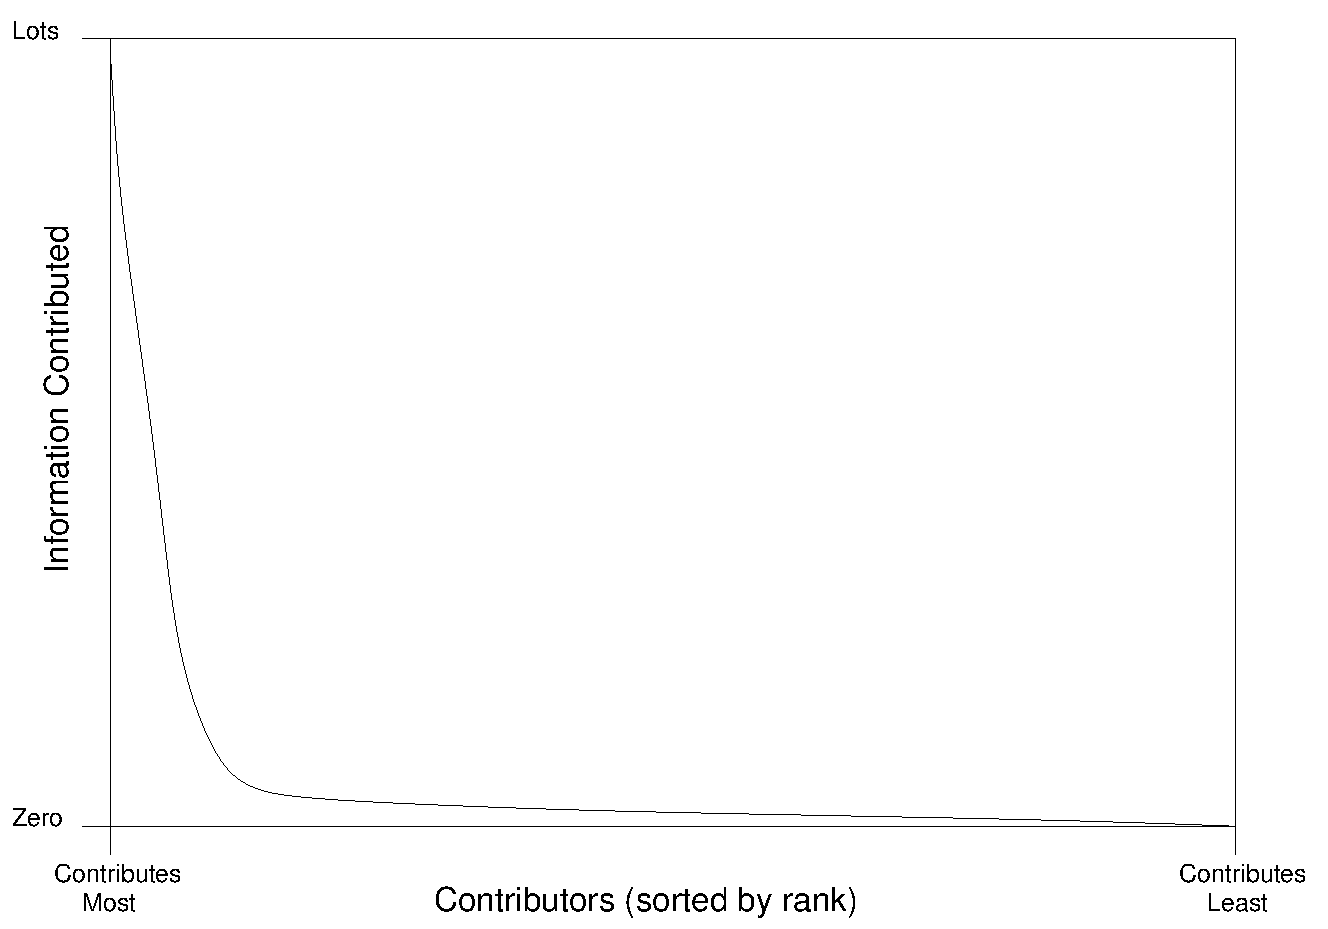
\includegraphics[width=0.7\textwidth]{figures/zipf_plot}
\end{center}

\end{frame}
%%%%%%%%%%%%%%%%%
\begin{frame}

\hspace{0.7in}Surveys don't use the \textcolor{blue}{fat-head} or the \textcolor{blue}{long-tail}

\begin{center}
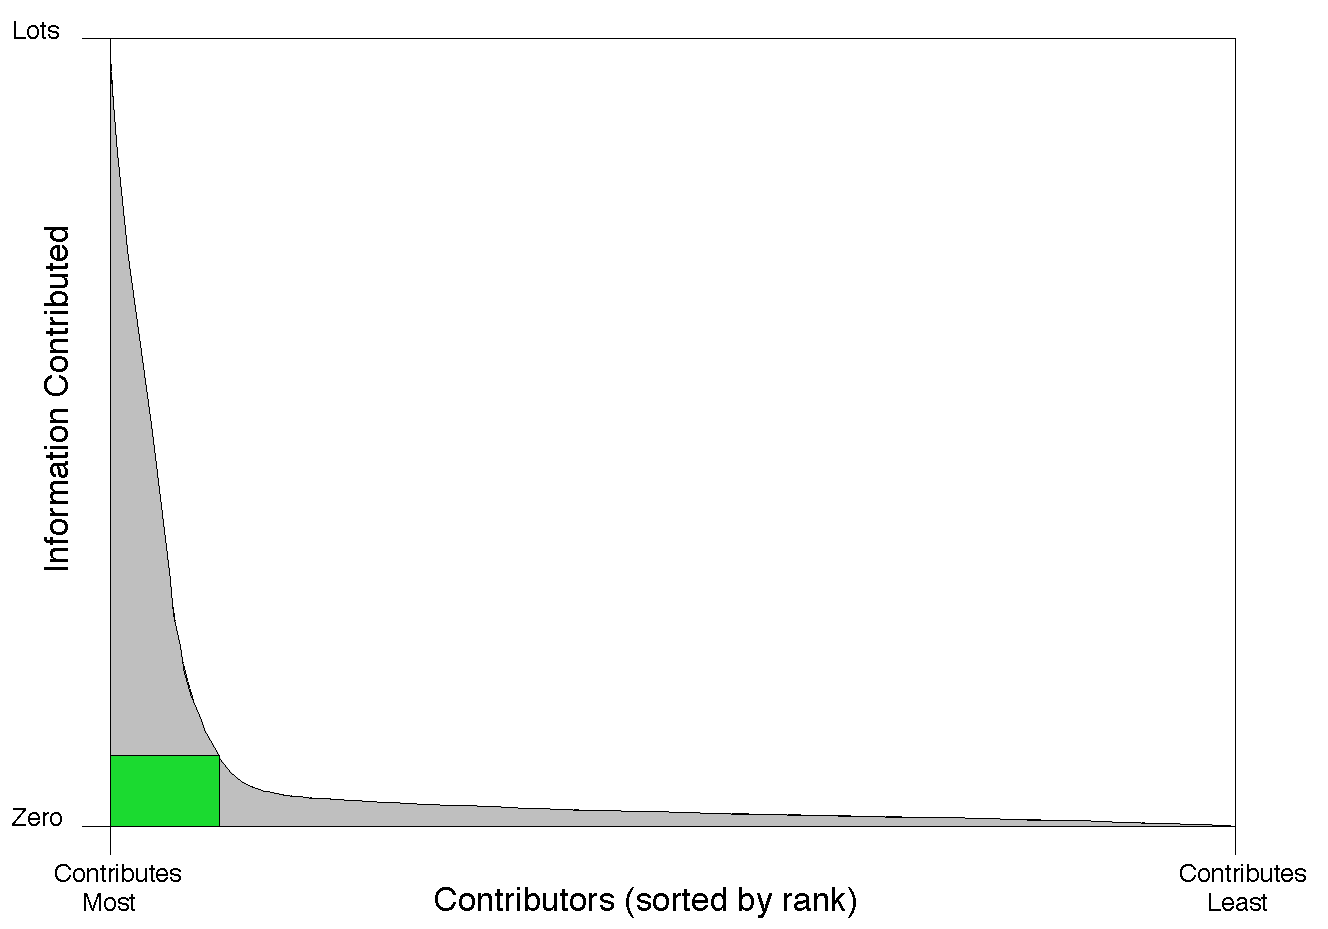
\includegraphics[width=0.8\textwidth]{figures/zipf_plot_withoverlay}
\end{center}

\end{frame}
%%%%%%%%%%%%%%%%%%
\begin{frame}

General principles of wiki surveys:
\begin{itemize}
\item greedy
\pause
\item collaborative
\pause
\item adaptive
\end{itemize}

\end{frame}
%%%%%%%%%%%%%%%%
\begin{frame}

\begin{center}
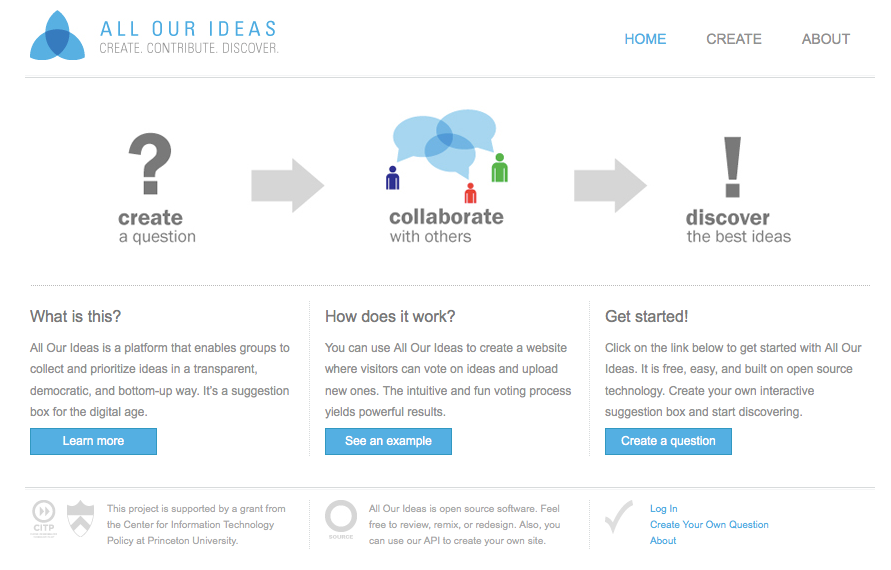
\includegraphics[width=0.9\textwidth]{figures/aoi_splash}
\end{center}

\end{frame}
%%%%%%%%%%%%%%%%%%
\begin{frame}

See Salganik and Levy (2015):
\begin{itemize}
\item full details of statistical model
\item case studies
\end{itemize}

\end{frame}
%%%%%%%%%%%%%%%%
\begin{frame}

\begin{center}
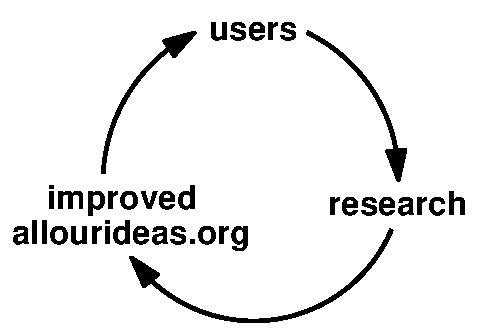
\includegraphics[width=0.6\textwidth]{figures/virtuous_cycle}
\end{center}

\end{frame}
%%%%%%%%%%%%%%%%
\begin{frame}

Currently hosting:\\
8,000 wiki surveys with 450,000 ideas and 13 million votes
\vf

\begin{center}
\begin{tabular}{m{1.4in} m{1.4in} m{1.4in}}

\includegraphics[width=1.2in]{figures/edemocracia} & 
\includegraphics[width=1.4in]{figures/ows_horizontal} & 
\includegraphics[width=1.3in]{figures/legg_mason_logo}\\
\vspace{0.2in}

\includegraphics[width=1.1in]{figures/un_logo_white_bkg} & 
\includegraphics[width=1in]{figures/200px-Wikipedia-logo} & 
\includegraphics[width=1.2in]{figures/harvard_business_publishing}
\end{tabular}
\end{center}

\end{frame}
%%%%%%%%%%%%%%%%%
\begin{frame}

\begin{itemize}
\item Questions about building it?
\item Questions about system-building as part of social research? (professional concerns?, kinds of things learned?)
\end{itemize}

\end{frame}
%%%%%%%%%%%%%%%%%


\end{document}
